\chapter{Analysis of Retract Force Curves in Colloidal Systems}

\section{Introduction}

\subsubsection{Analysis of Silica-silica retract curves}

In AFM, the study of force curves between silica surfaces in saline environments is a well explored avenue. However, the journey back from the surface — the retrace curve is often overlooked. Standard practice in AFM analysis tends to focus on the approach curves specifically, yet with every approach curve recorded, a corresponding retrace is inherently generated. However, a review of the literature reveals a conspicuous absence of retrace curve analysis; most studies emphasize the approach while relegating the retrace to a footnote, if it is acknowledged at all \cite{Retrace}. % \cite{John}.

This omission is understandable. Retrace curves can present a messier dataset, with the variability and complexity that derives from the chaotic nature of interactions when a tip withdraws from contact. This is due to a multitude of factors influencing the tip upon retraction: capillary forces, adhesion hysteresis, and tip contamination are but a few of the phenomena that can alter the tip's path back from the surface. While an approach curve starts from a place free of influence from the target in a stable part of a DLVO curve, the retrace starts at the point where it often is most complex.

Furthermore, DLVO theory, while capable in describing forces during the approach, can encounter hurdles when applied to the retrace curve. The symmetry of interaction predicted by DLVO when a tip approaches and retracts from a surface is often disrupted in practice. The retrace curve does not simply mirror the approach; it is influenced by history-dependent effects and irreversible changes to the tip or surface.

Within this chapter, we focus on these retrace curves, unpacking the generally noisier data in order to uncover the forces present between silica surfaces at the nanoscale. It is here where the complex analysis software shines, allowing conclusions to be drawn from curves that would otherwise be rejected.

The chapter advocates for a more holistic view in the field of AFM study, demonstrating that the insights gleaned from retrace curves are indispensable. By embracing the full cycle of approach and retraction, a more complete picture of the interaction forces at play can be derived. The retrace curve, often overlooked, may hold the key to a deeper understanding of surface interactions, and it is time we turn our attention to this pivotal part of the AFM narrative.

\section{MFP-1D contact force derivation}

This section will overview the results for the following LiCl concentrations: 0.6mM, 1.6mM, 5mM, 10mM, 25mM, 50mM, 230mM, 550mM. For each concentration multiple sites are analysed, highlighting features of each curve in preparation for analysis. The analytical approach to processing this large dataset is given in Chapter 4. 

The removal retrace curves followed the same reasoning in the previous chapter, and overlapped with the ones removed in the approach curves. This was largely due to machine errors (such as failing to connect to the surface) or from too little data within the window. The sheer volume of data more than made up for the removals however.

The graphs presented here have, once again, been meticulously selected from a broader dataset, chosen to demonstrate a good fit, to highlight the force profile and to elucidate the forces present between the interacting surfaces.

The optimization of data processing was informed by an extensive analysis of hundreds of thousands of curves. It is the same process laden with additional challenges, primarily due to the inherent noise and the diverse effects that can influence the tip upon retraction, such as capillary forces, adhesion hysteresis, or contamination. Ensuring accuracy in the retrace fit is important; a poor fit could yield erroneous curves and unreliable interpretations.

Three distinct graph types were chosen to demonstrate the fit for each of the concentrations. The retrace force curve, constructed from binned averages, depicts the aggregate behavior of the tip during retraction. Unlike its approach counterpart, the retrace curve tends to be much nosier in areas of adhesion, this is due to the variation in attractive forces within the same dataset.

The force versus the Z-piezo position reflects the forces at play as the tip disengages from the surface. It also highlights where the graph contact phase is determined.

The force histogram statistical compiles a distribution of the retrace forces encountered across multiple measurements. It provides a clear visual representation of the variability and the most probable forces during tip retraction. It also highlights the variability in the forces present.


\insertretractfigures{6}{0.6}{1}{}
\insertretractfigures{6}{0.6}{2}{}
\insertretractfigures{6}{0.6}{3}{}

0.6mM demonstrates the variability present in retrace curves. Occasionally, a retrace will have a higher attractive force. In general however, 0.6mM has very little to no attractive forces between the interacting elements.

%1.6
\insertretractfigures{6}{1.6}{1}{}
\insertretractfigures{6}{1.6}{2}{}

1.6mM has the same interesting shelf feature seen in the previous chapter. Interestingly - this shelf is largely in the same force range as the approach. Otherwise, 1.6 again has little attractive force, though notibly more than 0.6mM.

%5
\insertretractfigures{6}{5}{1}{}
\insertretractfigures{6}{5}{2}{}
\insertretractfigures{6}{5}{3}{}

5mM demonstrates that as the range of pull off forces increases, so too does the variability in the binned points in the average curve post fit. This is due to the range of distances the cantilieve disengages from the surface.

%10 2 sites
\insertretractfigures{6}{10}{1}{}
\insertretractfigures{6}{10}{2}{}
\insertretractfigures{6}{10}{3}{}

10mM starts to transition from a the occasional adhesive retrace curve, to a distribution of attractive ranges.Both site 2 and 3 have a a distribution similar to a normal distribution, unlike its predecessors.

%25 3 sites
\insertretractfigures{6}{25}{1}{}
\insertretractfigures{6}{25}{2}{}
\insertretractfigures{6}{25}{3}{}

25mM realises the previous observation, with a more frequent distribution of a range of attractive forces. As a result, the summed data is very noisy.

%50 2 sites
\insertretractfigures{6}{50}{1}{}
\insertretractfigures{6}{50}{2}{}

%230 2 sites
\insertretractfigures{6}{230}{1}{}
\insertretractfigures{6}{230}{2}{}

230mM starts to have a more coherent attractive profile as the theory starts to transition into a more attractive profile between the surfaces.

%550 3 sites
\insertretractfigures{6}{550}{1}{}
\insertretractfigures{6}{550}{2}{}
\insertretractfigures{6}{550}{3}{}

\section{Overall force vs LiCl concentration graphs}

The pull off forces calculated were subsequently averaged, with the standard deviation calculated using equation \ref{eq:Stdevavg}.

\begin{figure}
    \centering
    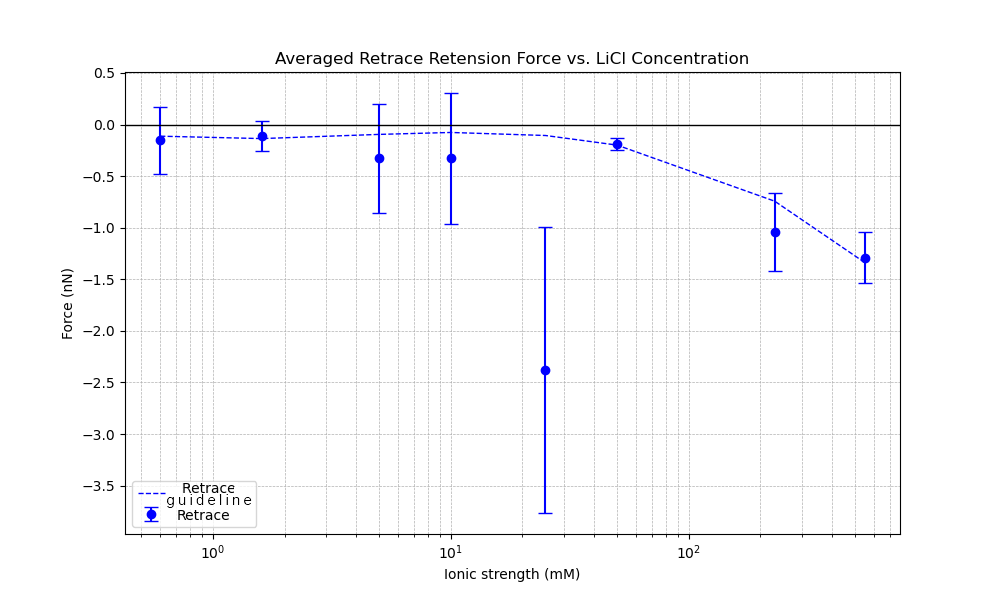
\includegraphics[width=1\linewidth]{chapter6/Averages.png}
    \caption{Site one calculated attractive force retained from contact with standard deviation error bars.}
    \label{fig:site1cont}
\end{figure}


The retrace curve shown in figure \ref{fig:site1cont} represent the attractive forces that are retained when the AFM tip is retracted from the contact with the surface at different LiCl concentrations. The retrace curve shows an attractive force plateu, until a critical concentration at around 50mM where the attractive force between the tip and surface increases increasing LiCl concentration, with the force generally following a trend downwards. However 25mM is perplexing, as it demonstrates the strongest attractive force, though it is worth noting that 25mM was also a bit of an oddity in the approach curves due to it's higher standard deviation. This could be due to other reasons, such as a unexpected surface perturbation providing additional friction. In general, however, there is a trend of increasing attractive force past 50mM concentration, and thus pull off force across the datapoints.

Another aspect that stands out is the prominence of the standard deviation, especially at the higher concentrations. This is typical for retrace curves due to the reasons mentioned earlier such as tip changes upon contact. It is also interesting to note that the attractive forces in retrace curves are usually not symmetrical with the approach curves due to various interactions that can occur when the tip is in contact with the surface. These interactions include adhesion hysteresis, capillary forces, and possible tip contamination or wear, which can all affect the tip as it retracts and lead to the variability observed.

One final interesting note is the observation of the 50mM tipping point present in both the approach and retrace curve, indicating that past 50mM there potentially could be some kind of mechanism that impacts the electrostatic repulsion, rather than a linear build up of ions on the surface (potentially enough ions to fully saturate the surface?).

This analysis is important for interpreting the overall behavior of the system and for validating models of interfacial forces, which is the focus of our next chapter.